\chapter{The Backend}
\label{backend}
	\section{Introduction}
		\begin{figure}[H]
			\iftrue
			\caption{Backend Services}
			\centering
			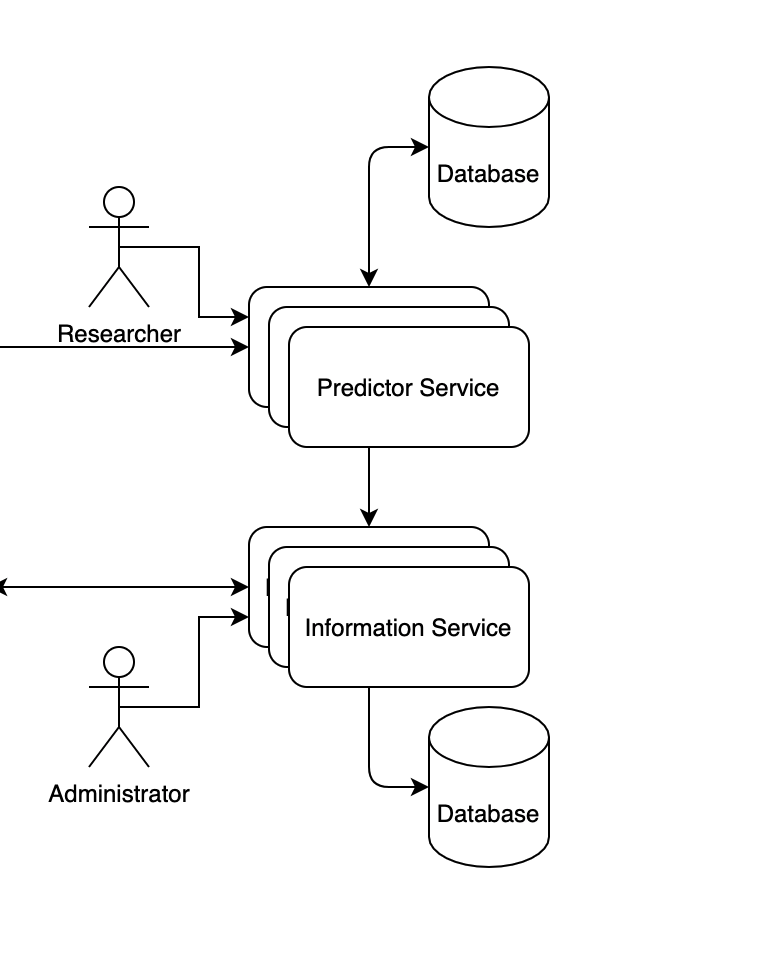
\includegraphics[scale=0.5]{figures/backend}
			\fi
		\end{figure}
		This chapter will cover extensively the inner workings of the backend services, namely the Information and the Prediction services.
		We will go through their internal architectures as well as some key areas of interest.
	\section{Information Service}
		The Information Service(internally known as uortmc-infobe) is the service that handles the information of our entities, 
		namely the patients, the scans, the end-users, and their interconnections. Additionally, it handles authentication and 
		includes the notification system, capable of notifying a given end-user for the completion of their tasks.
		\subsection{Technology Stack}
			The Information service uses several libraries to achieve its goals; the most important ones are listed below.
			\begin{itemize}
				\item Django framework
				\item psycopg2 database driver
			\end{itemize}	
			\subsubsection{Django Framework}
				\label{django}
				
				Django is a free and open-source, python based web framework that uses the model-template-view(MTV) architecture pattern.  
				It is maintained by an American non-profit organization called Django Software Foundation (DSF). 
				Django offers the code infrastructure to develop RESTFul[\cite{restful-rfc7231}] microservices with ease, and it is the backbone 
				of both of our microservices.
			\subsubsection{psycopg2 database driver}
				\label{psycopg2}
				psycopg2 is a famous Postgres database driver for python. psycopg2 offers the interface for our Postgres database connection, implementing 
				the server-client protocol behind the scenes.
		\subsection{Code Architecture}
			The Information service is designed to be a fully Object Oriented Entity[\cite{oop}].
			The architectural design of the Information Service can be seen below.\pagebreak
			\begin{figure}[H]
				\iftrue
				\caption{OOP Diagram}
				\centering
				 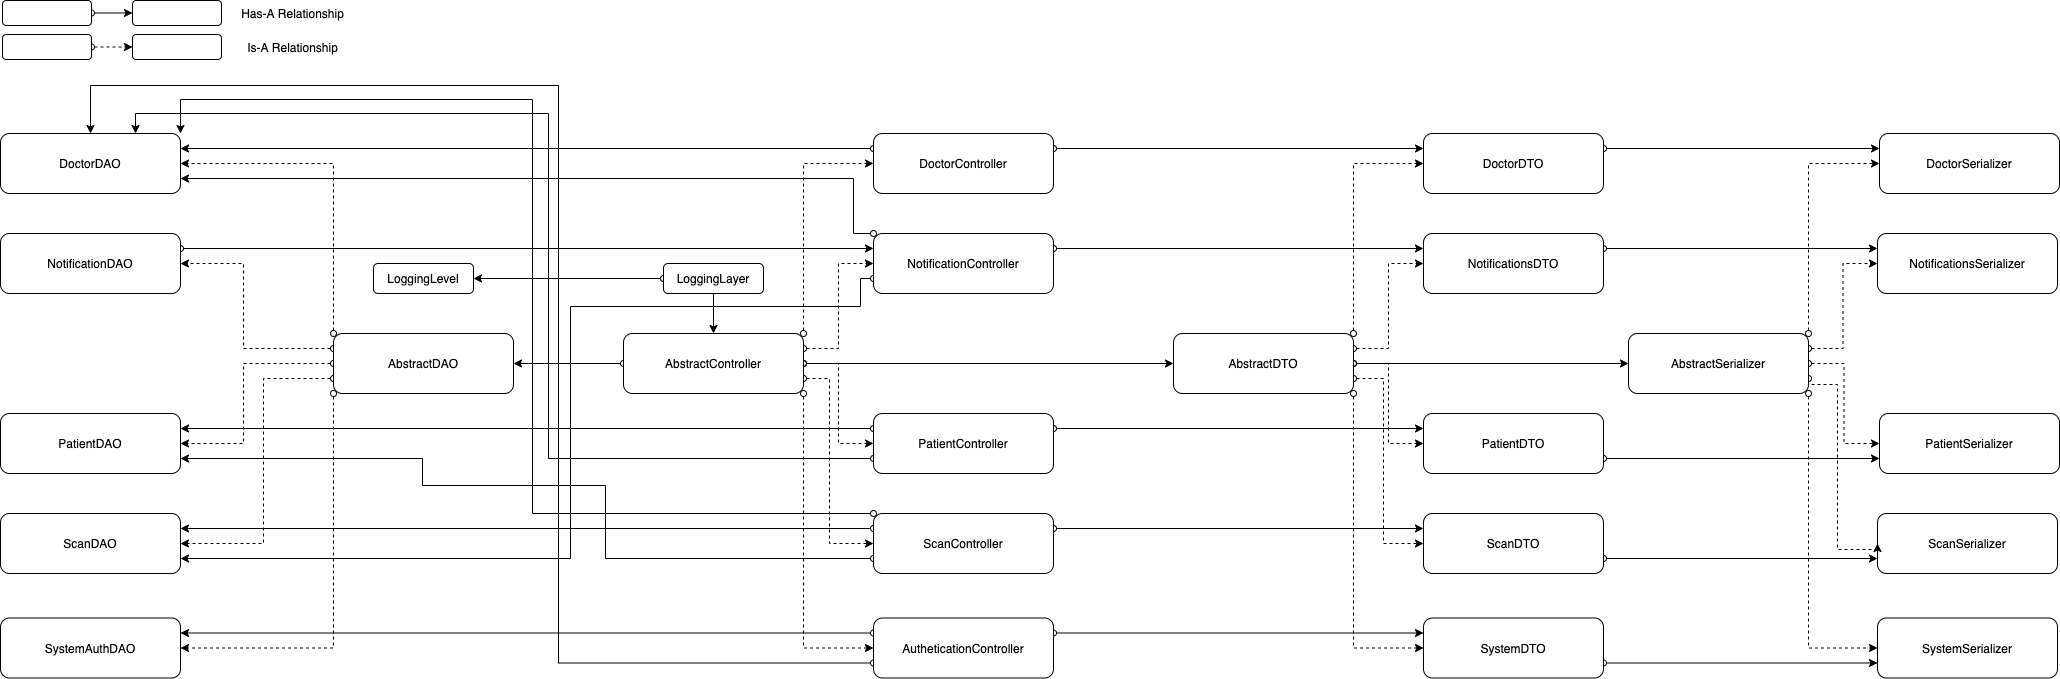
\includegraphics[angle=90,origin=c,scale=0.3]{figures/InformationServiceArchitecture}
				\fi
			\end{figure}\pagebreak
			The following classes are serving as endpoints to requests
			\begin{itemize}
				\item \textbf{DoctorController}: This Class handles everything related to the Doctor Entity.
				\item \textbf{NotificationController} : This Class handles everything related to the Notification Entity.
				\item \textbf{PatientController} : This Class handles everything related to the Patient Entity.
				\item \textbf{ScanController} : This Class handles everything related to the Scan Entity.
				\item \textbf{AutheticationController} : This Class handles everything related to the Authentication service.
			\end{itemize}
			When a request is sent to the Information service, the proper class is selected based on the request endpoint and details. 
			Then the respective class will use the rest of the class's services to perform the needed actions and respond to the 
			request accordingly. An exhaustive list of the significant classes is given below.
			\begin{center}
				\begin{tabular}{ |c|c| } 
					\hline
					DoctorDAO & Handles the SQL Queries of Doctor Entity \\
					NotificationDAO & Handles the SQL Queries of Notification Entity  \\\
					PatientDAO & Handles the SQL Queries of the Patient Entity\\
					ScanDAO & Handles the SQL Queries of the Scan Entity\\
					SystemAuthDAO & Handles the SQL Queries of the Authentication service\\
					AbstractDAO & Used to describe any DAO(Data Access Object) available\\
					LoggingLayer & Used by controllers to notify the operator in case of errors\\
					LoggingLevel &Used by LoggingLayer to describe the severity of an error\\
					AbstractController & Used to describe any controller available\\
					AbstractDTO & Used to describe any DTO(Data Transfer Object)'s available\\
					DoctorDTO & The responce objects for Doctor Entities\\
					NotificationsDTO & The responce objects for Notification Entities\\
					PatientDTO & The responce objects for Patient Entities\\
					ScanDTO & The responce objects for Scan Entities\\
					SystemDTO & The responce objects for Authentication Entities\\
					AbstractSerializer & Used to describe any serializer available\\
					DoctorSerializer & Used to convert Doctor DTO responce into JSON\\
					NotificationsSerializer & Used to convert Notification DTO responce into JSON\\
					ScanSerializer & Used to convert Scan DTO responce into JSON\\
					SystemSerializer & Used to convert SystemAuthDTO responce into JSON\\
					\hline
				\end{tabular}
			\end{center}
		\subsection{Information Service Database}
			\label{postgres}
			
			The Information Service uses an RDBMS(Relational Database Management System)[\cite{friedrichsen_ruffolo_monk_starks_pratt_last_1995}] called Postgres. PostgreSQL is an open-source and free 
			relational database emphasizing extensibility and SQL standard compliance. The relational diagram of the Information Service can be 
			seen below. Additional information relating to the E-R Diagram can be found in chapter \ref{entity-relation-analysis})\pagebreak
			\begin{figure}[H]
				\iftrue
				\caption{E-R Diagram}
				\centering
				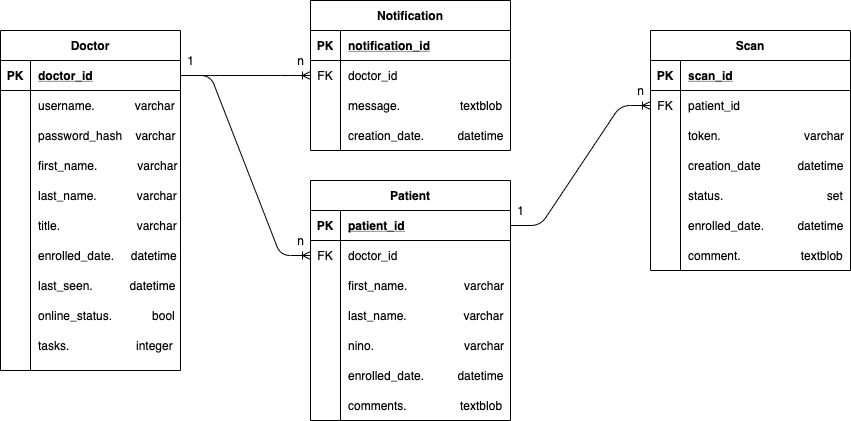
\includegraphics[angle=90,origin=c,scale=0.8]{figures/InformationServiceDatabaseDiagram}
				\fi
			\end{figure}\pagebreak
	
	\section{Prediction Service}
		The Prediction Service(internally known as uortmc-taskbe) is the service that handles the prediction process of ultrasound 
		images; it also has the responsibility of notifying the end-user when a task is completed by calling the Information Service's 
		Notification service. In this section, we will briefly look at the Prediction Service internals, except the prediction itself. 
		For more information on the prediction process, please refer to chapter \ref{prediction-process}.
		\subsection{Technology Stack}
			The Prediction service uses several libraries to achieve its goals, and the most important ones are listed below.
			\begin{itemize}
				\item Django framework (see paragraph \ref{django})
				\item psycopg2 database driver (see paragraph \ref{psycopg2})
				\item base64 decoders
				\item imghdr image library
				\item Pykka actors
			\end{itemize}
			\subsubsection{base64 decoder}
				base64 decoding library is a famous decoding library for python. It offers the capability of encoding and decoding 
				messages in base64 format. We use this library for the ultrasound image scan transmission from the frontend application 
				into the predictor service.
			\subsubsection{imghdr image library}
				imghdr library provides the capability of the Prediction service to recognize if a given image is corrupted or not.
			\subsubsection{Pykka Actors library}
				"Pykka is a Python implementation of the actor model[\cite{hewitt2015actor}]. The actor model introduces some 
				simple rules to control the sharing of state and cooperation between execution units, making it easier to build 
				concurrent applications."[\cite{magnus_2010}] Pykka actors are used extensively on the Prediction service, 
				especially on the prediction algorithms themselves, making the service capable of working as a distributed 
				system with multiple nodes, working together when the workload is higher(for more information, please refer to 
				paragraph \ref{flexible-scaleability-factor}).
				
		\subsection{Code Architecture}
			The Prediction service is designed to be a fully Object Oriented Entity[\cite{oop}].
			The architectural design of the Prediction Service can be seen below.\pagebreak
			\begin{figure}[H]
				\iftrue
				\caption{OOP Diagram}
				\centering
				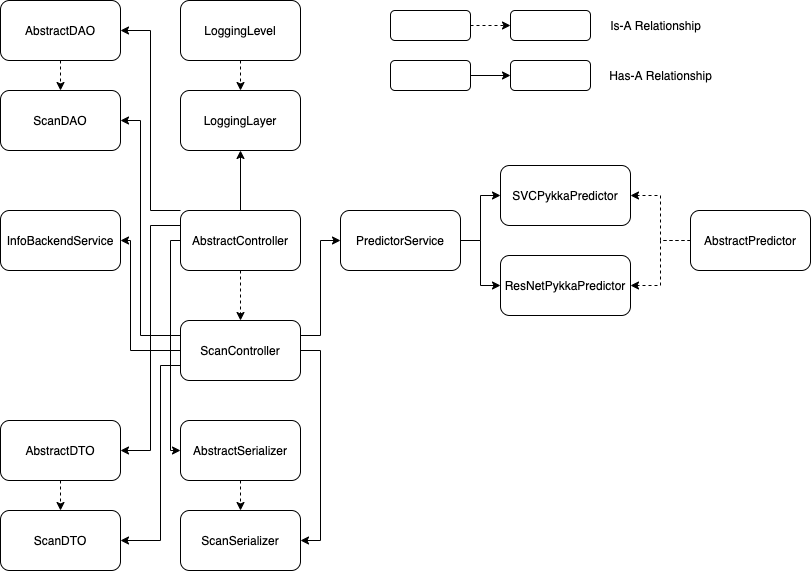
\includegraphics[angle=90,origin=c,scale=0.7]{figures/PredictorServiceCodeDiagram}
				\fi
			\end{figure}\pagebreak
			When a request is sent to the Predictor service, an object from class ScanController takes the responsibility 
			of handling the request. Then the ScanController will use the rest of the classes and objects services to perform
			 the needed actions and respond to the request appropriately. An exhaustive list of the significant rest classes is 
			 given below.
			\begin{center}
				\begin{tabular}{ |c|c| } 
					\hline
					AbstractDAO & Used to describe any DAO(Data Access Object) available \\
					ScanDAO & Handles the SQL Queries of Scan Entity  \\\
					InfoBackendService & Handles the communications between Predictor and Information Services\\
					AbstractDTO & Used to describe any DTO(Data Transfer Object)'s available\\
					ScanDTO & The responce object for Scan Entities\\
					LoggingLevel &Used by controllers to notify the operator in case of errors\\
					LoggingLayer & Used by LoggingLayer to describe the severity of an error\\
					AbstractController & Used to describe any Controller available\\
					AbstractSerializer &  Used to describe any serializer available\\
					ScanSerializer & Used to convert Scan DTO responce into JSON\\
					PredictorService & Handles the prediction of the ultrasound images\\
					SVCPykkaPredictor & Handles the predictions using the SVC Algoritm(refer to chapter\ref{prediction-process})\\
					ResNetPykkaPredictor & Handles the predictions using the RESNet Algoritm(refer to chapter\ref{prediction-process})\\
					AbstractPredictor & Used to describe any Predictor available\\
					\hline
				\end{tabular}
			\end{center}
		\subsection{Prediction Service Database}
		
			The Predictor Service uses an RDBMS(Relational Database Management System)[\cite{friedrichsen_ruffolo_monk_starks_pratt_last_1995}] called Postgres(for more information, please 
			refer to paragraph \ref{postgres}). The relational diagram of the Predictor Service can be seen below. Additional information relating to 
			the E-R Diagram can be found in the chapter \ref{entity-relation-analysis}.
			\begin{figure}[H]
				\iftrue
				\caption{E-R Diagram}
				\centering
				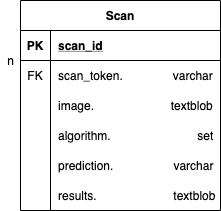
\includegraphics[scale=0.6]{figures/PredictorServiceDatabaseDiagram}
				\fi
			\end{figure}
		
		
			
		